\documentclass[14pt]{extarticle}

\usepackage[margin=0.5in]{geometry}
\usepackage{pgfplots}
\usepackage{multicol}
\usepackage{gensymb}

\pgfplotsset{compat=newest}

\title{EE-220 Homework 6}
\author{Jonathan Forhan}
\date{ }

\renewcommand{\thesubsection}{\thesection-\alph{subsection}}

\begin{document}
\maketitle

\boldmath
\section{Using \textit{dot products}, find the \textit{interior angles} of the triangle defined by the following points: \newline
  $A(2,0,2)$, $B(-3,-3,5)$, $C(5,1,0)$.}
\unboldmath{$ $}

\begin{center}
	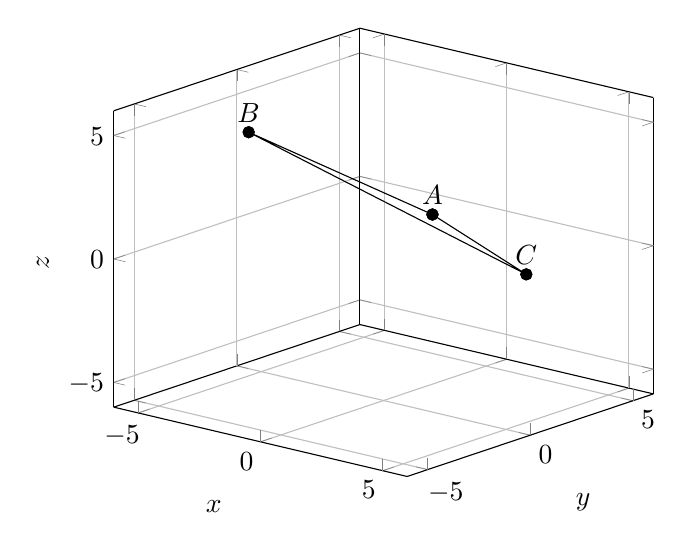
\begin{tikzpicture}
		\begin{axis}[
				view={40}{20},
				grid=both,
				xmax=6,
				ymax=6,
				zmax=6,
				xmin=-6,
				ymin=-6,
				zmin=-6,
				xlabel=$x$,
				ylabel=$y$,
				zlabel=$z$,
			]
			\addplot3[color=black,mark=*,mark size=2] table[row sep=crcr] {
					2 0 2 \\
					-3 -3 5 \\
					5 1 0 \\
					2 0 2 \\
				};
			\addplot3[mark=*,black,point meta=explicit symbolic,nodes near coords] coordinates {(2,0,2)[$A$]};
			\addplot3[mark=*,black,point meta=explicit symbolic,nodes near coords] coordinates {(-3,-3,5)[$B$]};
			\addplot3[mark=*,black,point meta=explicit symbolic,nodes near coords] coordinates {(5,1,0)[$C$]};
		\end{axis}
	\end{tikzpicture}
\end{center}
% Angle A
\[
	\overrightarrow{AB}\cdot\overrightarrow{AC}=|\overrightarrow{AB}||\overrightarrow{AC}|\cos(\theta)=
	\left(-5\vec{a}_x-3\vec{a}_y+3\vec{a}_z\right)\cdot\left(3\vec{a}_x+\vec{a}_y-2\vec{a}_z\right)=-24
\]
\[
	\angle{A}=\cos^{-1}\left(\frac{\overrightarrow{AB}\cdot\overrightarrow{AC}}{|\overrightarrow{AB}||\overrightarrow{AC}|}\right)=
	\cos^{-1}\left(\frac{-24}{\sqrt{43}\sqrt{14}}\right)=168.01\degree
\]
% Angle B
\[
	\overrightarrow{BA}\cdot\overrightarrow{BC}=|\overrightarrow{BA}||\overrightarrow{BC}|\cos(\theta)=
	\left(5\vec{a}_x+3\vec{a}_y-3\vec{a}_z\right)\cdot\left(8\vec{a}_x+4\vec{a}_y-5\vec{a}_z\right)=67
\]
\[
	\angle{B}=\cos^{-1}\left(\frac{\overrightarrow{BA}\cdot\overrightarrow{BC}}{|\overrightarrow{BA}||\overrightarrow{BC}|}\right)=
	\cos^{-1}\left(\frac{67}{\sqrt{43}\sqrt{105}}\right)=4.35\degree
\]
% Angle C
\[
	\overrightarrow{CA}\cdot\overrightarrow{CB}=|\overrightarrow{CA}||\overrightarrow{CB}|\cos(\theta)=
	\left(-3\vec{a}_x-\vec{a}_y+2\vec{a}_z\right)\cdot\left(-8\vec{a}_x-4\vec{a}_y+5\vec{a}_z\right)=38
\]
\[
	\angle{C}=\cos^{-1}\left(\frac{\overrightarrow{CA}\cdot\overrightarrow{CB}}{|\overrightarrow{CA}||\overrightarrow{CB}|}\right)=
	\cos^{-1}\left(\frac{38}{\sqrt{14}\sqrt{105}}\right)=7.64\degree
\]

\clearpage

\boldmath
\section{Consider the flux density $\vec{D}=2\rho\vec{a}_\rho+\sin(\phi)\vec{a}_z\left[\frac{\mathrm{C}}{\mathrm{m}^2}\right]$.}
\unboldmath{$ $}

\boldmath
\subsection{Calculate the total eletric flux passing through the surface defined by $1\le\rho\le3$, $0\le\phi\le \pi$, $z=4$.}
\unboldmath{$ $}

\[
	\Psi=\int_v\vec{\nabla}\cdot\vec{D}dv
\]
\[
	\vec{\nabla}\cdot\vec{D}=\frac{1}{\rho}\frac{\partial(\rho D_\rho)}{\partial\rho}+\frac{1}{\rho}\frac{\partial D_\phi}{\partial\phi}+\frac{\partial D_z}{\partial z}
\]
\[
	\vec{\nabla}\cdot\vec{D}=\frac{1}{\rho}\frac{\partial(2\rho^2)}{\partial\rho}=\frac{1}{\rho}(4\rho)=4
\]
\[
	\Psi=\int_v 4 dv=\int_{z=4}^{z=4}\int_{\phi=0}^{\phi=\pi}\int_{\rho=1}^{\rho=3}4\rho d\rho d\phi dz = 0
\]

\boldmath
\subsection{Find the \textit{eletric field intensity} $\vec{E}$.}
\unboldmath{$ $}

\[
	\vec{E}=\frac{\vec{D}}{\epsilon_0} = \frac{2\rho}{\epsilon_0}\vec{a}_\rho+\frac{\sin(\phi)}{\epsilon_0}\vec{a}_z\left[\frac{\mathrm{V}}{\mathrm{m}}\right]
\]

\clearpage

\boldmath
\section{Assuming $\vec{D}=r\vec{a}_r-\cos(\phi)\vec{a}_\theta+\sin^2(\theta)\vec{a}_\phi\left[\frac{\mathrm{C}}{\mathrm{m}^2}\right]$, \newline
  calculate the electric flux through both surfaces of the hemisphere of radius 2 and $0\le\theta\le\frac{\pi}{2}$.}
\unboldmath{$ $}

\[
	\Psi=\int_v\vec{\nabla}\cdot\vec{D}dv
\]
\[
	\vec{\nabla}\cdot\vec{D}=\frac{1}{r^2}\frac{\partial(r^2 D_r)}{\partial r}+\frac{1}{r\sin{\theta}}\frac{\partial (D_\theta\sin{\theta})}{\partial\theta}+\frac{1}{r\sin{\theta}}\frac{\partial D_\phi}{\partial\phi}
\]
\[
	\vec{\nabla}\cdot\vec{D}=\frac{1}{r^2}\frac{\partial(r^3)}{\partial r}+\frac{1}{r\sin{\theta}}\frac{\partial (-\cos{\phi}\sin{\theta})}{\partial\theta}+\frac{1}{r\sin{\theta}}\frac{\partial \sin^2{\theta}}{\partial\phi}
\]
\[
	\vec{\nabla}\cdot\vec{D}=\frac{3r^2}{r^2}+\frac{-\cos{\phi}\cos{\theta}}{r\sin{\theta}}
\]
\[
	\Psi=\int_v \left(\frac{3r^2}{r^2}+\frac{-\cos{\phi}\cos{\theta}}{r\sin{\theta}}\right)dv=
\]
\[
	\int_{\phi=0}^{\phi=\pi}\int_{\theta=0}^{\theta=\frac{\pi}{2}}\int_{r=0}^{r=2}\left(\frac{3r^2}{r^2}+\frac{-\cos{\phi}\cos{\theta}}{r\sin{\theta}}\right)r^2\sin{\theta}dr d\theta d\phi=
\]
\[
	\int_{\phi=0}^{\phi=\pi}\int_{\theta=0}^{\theta=\frac{\pi}{2}}\int_{r=0}^{r=2}\left(3r^2\sin\theta-r\cos{\phi}\cos{\theta}\right)dr d\theta d\phi
\]

\[
	\int_{\theta=0}^{\theta=\frac{\pi}{2}}\int_{r=0}^{r=2}\left(3r^2\sin\theta(\phi)-r\sin\phi\cos\theta\right)dr d\theta \bigg|_0^{\pi}
\]
\[
	\int_{\theta=0}^{\theta=\frac{\pi}{2}}\int_{r=0}^{r=2}\left(3\pi r^2\sin\theta-r\cos{\theta}\right)dr d\theta
\]
\[
	\int_{r=0}^{r=2}\left(-3\pi r^2\cos\theta-r\sin\theta\right)dr \bigg|_0^{\pi / 2}
\]
\[
	\int_{r=0}^{r=2}\left(-r+3\pi r^2\right)dr
\]
\[
	\left(-\frac{r^2}{2}+\pi r^3\right)dr \bigg|_0^2
\]
\[
	\Psi=8\pi-2=23.13
\]

\end{document}
